%
% This work is licensed under a Creative Commons Attribution-ShareAlike 4.0 International License.
% http://creativecommons.org/licenses/by-sa/4.0/
%

% DO NOT COMPILE THIS FILE DIRECTLY!
% This is included by the other .tex files.


\begin{frame}
    
\includegraphics[scale=.3]{images/logo-circl-Forensics.png}
    \begin{itemize}
        \item[]
        \item[]
        \item[] 1. Windows Registry
    \end{itemize}
\end{frame}


\begin{frame}[fragile]
  \frametitle{1.1 About: Windows Registry}
    \begin{itemize}
        \item MS DOS and old Windows
            \begin{itemize}
                \item On system boot: What programs to load
                \item How the system interact with the user
                \begin{itemize}
			\item[] $\to$ \texttt{autoexec.bat}
			\item[] $\to$ \texttt{config.sys}
			\item[] $\to$ \texttt{system.ini}
			\item[] $\to$ \texttt{win.ini}
                \end{itemize}
            \end{itemize}
        \item \url{https://support.microsoft.com/en-us/help/256986/}
            \begin{itemize}
                \item A central hierarchical database
                \item Replace text based config files
                \item Contains information for operating
                \begin{itemize}
                    \item Hardware in the system
                    \item All aspects of MS Windows
                    \item Installed applications
                    \item Each user
                \end{itemize}
            \end{itemize}
    \item[] $\to$ A gold mine for forensics
    \end{itemize}
\end{frame}


\begin{frame}[fragile]
  \frametitle{1.1 About: Windows Registry}
    \begin{figure}
        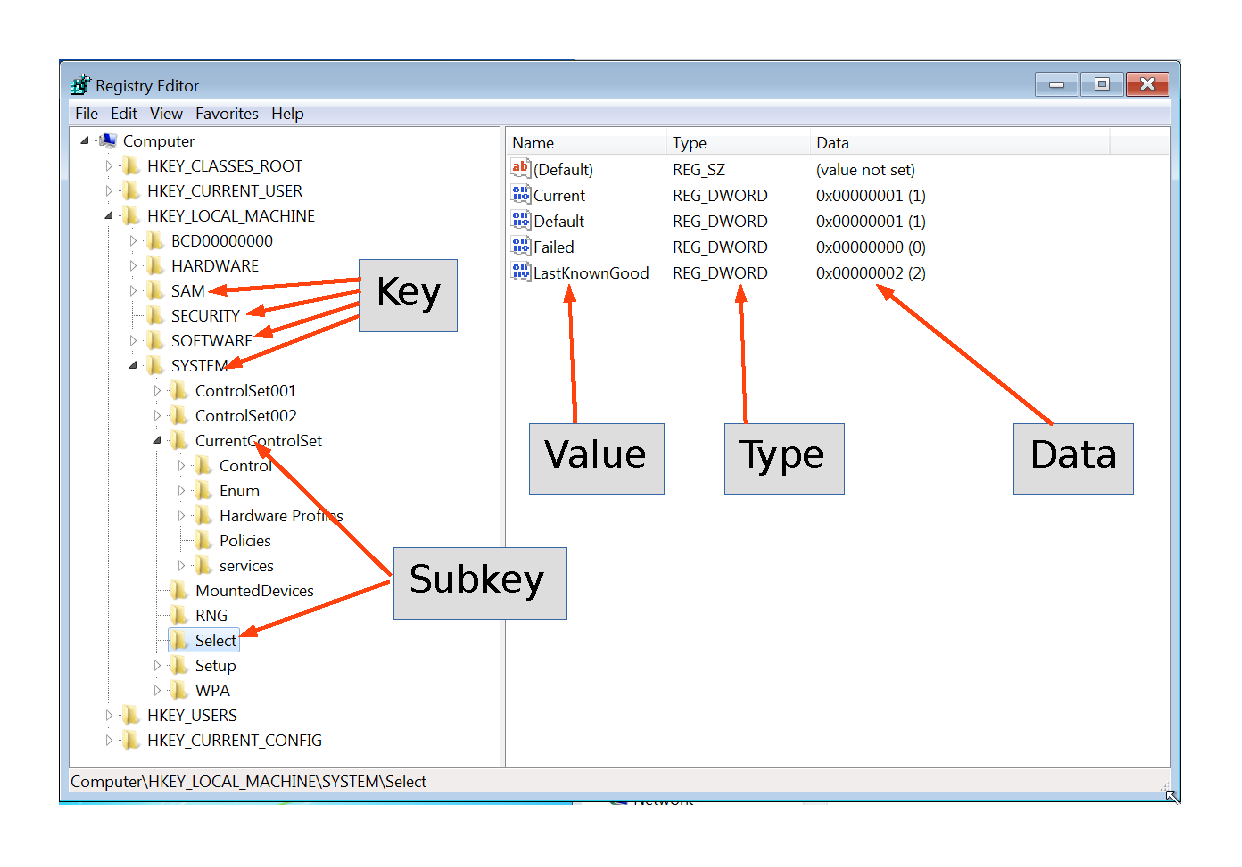
\includegraphics[scale=0.43]{images/nomenclature.pdf}
        \captionsetup{labelformat=empty,labelsep=none}
        \transparent{0.9}%
        \caption[]{\tiny Key data structures contains a last write time stamp}
    \end{figure}
\end{frame}


\begin{frame}[fragile]
  \frametitle{1.1 About: Windows Registry}
    \begin{itemize}
        \item Do you ever touch the Registry?
            \begin{itemize}
		\item \texttt{regedit.exe}
                \item Black Magic for many admins
		\item[] $\to$ Every user interacts with the Registry
		\item[]
            \end{itemize}
        \item Location of the hive files
            \begin{itemize}
                \item[] \begin{verbatim}%SystemRoot%\system32\config\end{verbatim}
                \item[] $\to$ \texttt{SAM, SECURITY, SYSTEM, SOFTWARE}
                \item[] \begin{verbatim}%UserProfile%\NTUSER.DAT\end{verbatim}
                \item[] \begin{verbatim}%UserProfile%\AppData\Local\Microsoft\Windows\UsrClass.dat\end{verbatim}
		\item[]
            \end{itemize}
        \item Timestamps $\to$ Timeline
    \end{itemize}
\end{frame}


\begin{frame}[fragile]
  \frametitle{1.2 Under the hood: Key Cell}
  \definecolor{light-gray}{gray}{0.70}
  \begin{lstlisting}[basicstyle=\tiny,escapechar=§]
     0000:  §\colorbox{light-gray}{a0ff ffff}§ 6e6b 2000  6f0f 0e3b b78d d101  ....nk .o..;....
     0010:  0200 0000 085e 0500  0000 0000 0000 0000  .....^..........
     0020:  ffff ffff ffff ffff  0200 0000 0021 0500  .............!..
     0030:  102e 0000 ffff ffff  0000 0000 0000 0000  ................
     0040:  1400 0000 1000 0000  0000 0000 0a00 0000  ................
     0050:  496e 7465 7266 6163  6573 0080 0200 0000  Interfaces......
  \end{lstlisting}
  \begin{lstlisting}[basicstyle=\tiny]
 Offsets:    0x00       0       4        Size
             0x04       4       2        Node ID
             0x06       6       2        Node type
             0x08       8       8        Last write time
                  ...      ...
             0x4c      76       2        Lenght of key name
             0x50      80     <76>       key name + padding
  \end{lstlisting}
  \begin{itemize}
      \item Exercise: Calculate the size of the key cell
      \begin{itemize}
          \item[] \texttt{a0 ff ff ff}
          \item[]
      \end{itemize}
      \item Exercise: Calculate the size of the key name
      \begin{itemize}
          \item[] \texttt{0a 00}
      \end{itemize}
  \end{itemize}
\end{frame}


\begin{frame}[fragile]
  \frametitle{1.2 Under the hood: Value Cell}
  \definecolor{light-gray}{gray}{0.70}
  \begin{lstlisting}[basicstyle=\tiny,escapechar=§]
     0000:                        §\colorbox{light-gray}{d8ff ffff}§ 766b 0d00          ....vk..
     0010:  0400 0080 0200 0000  0400 0000 0100 0000  ................
     0020:  4c61 7374 4b6e 6f77  6e47 6f6f 6400 0000  LastKnownGood...
  \end{lstlisting}
  \begin{lstlisting}[basicstyle=\tiny]
 Offset:     0x00       0       4        Size
             0x04       4       2        Node ID
             0x06       6       2        Value name length
             0x08       8       4        Data lenght
             0x0c      12       4        Data offset
             0x10      16       4        value typw
  \end{lstlisting}
  \begin{itemize}
      \item Exercise: Calculate the size of the value cell
      \begin{itemize}
          \item[] \texttt{d8 ff ff ff}
          \item[]
      \end{itemize}
      \item Exercise: Calculate the size of the value name length
      \begin{itemize}
          \item[] \texttt{0d 00}
      \end{itemize}
  \end{itemize}
\end{frame}


\begin{frame}[fragile]
  \frametitle{1.3 Hive files}
   \begin{itemize}
       \item[]
   \begin{itemize}
      \item SAM
      \begin{itemize}
          \item Local users
      \end{itemize}
      \item Security
      \begin{itemize}
          \item Audit settings
          \item Machine, domain SID
      \end{itemize}
      \item System
      \begin{itemize}
          \item General system configuration
          \item Networking, Auto run
          \item Program execution
          \item USB devices
       \end{itemize}
      \item Software
      \begin{itemize}
          \item Windows version, Profiles list
          \item Networking, Auto run
          \item Shell extensions, Browser helper objects
          \item Scheduled Tasks
          \item Program execution
      \end{itemize}
   \end{itemize}
   \end{itemize}
\end{frame}


\begin{frame}[fragile]
  \frametitle{1.3 Hive files}
    \begin{itemize}
        \item Windows XP:
        \item[] \begin{verbatim}C:\Documents and Settings\<username>\NTUSER.DAT\end{verbatim}
        \item[] \begin{verbatim}C:\Documents and Settings\<username>\Local Settings\\end{verbatim}
        \item[] \begin{verbatim}   Application Data\Microsoft\Windows\UsrClass.dat\end{verbatim}
        \item[]
        \item Windows Vista and above:
        \item[] \begin{verbatim}C:\Users\<user>\NTUSER.DAT\end{verbatim}
        \item[] \begin{verbatim}C:\Users\<user>\AppData\Local\Microsoft\Windows\\end{verbatim}
        \item[] \begin{verbatim}   UsrClass.dat\end{verbatim}
        \item[]
        \item \begin{verbatim}C:\Windows\inf\setupapi.log\end{verbatim}
    \end{itemize}
\end{frame}


\begin{frame}[fragile]
  \frametitle{1.4 RegRipper}
  \begin{itemize}
      \item Extract specific key values
  \begin{lstlisting}[basicstyle=\tiny]
$ rip.pl -p compname -r SYSTEM
	ComputerName    = WIN7WS
	TCP/IP Hostname = Win7WS
  \end{lstlisting}
      \item Alternative method
  \begin{lstlisting}[basicstyle=\tiny]
$ wine rip.exe -p compname -r SYSTEM
	ComputerName    = WIN7WS
	TCP/IP Hostname = Win7WS
  \end{lstlisting}
      \item RegRipper plugins
  \begin{lstlisting}[basicstyle=\tiny]
$ ls -l /usr/share/regripper/plugins | wc -l
	397
  \end{lstlisting}
      \item Ripping hive files with profiles
  \begin{lstlisting}[basicstyle=\tiny]
$ rip.exe -f sam -r SAM > out/sam.txt
$ rip.exe -f security -r SECURITY > out/security.txt
$ rip.exe -f system -r SYSTEM > out/system.txt
$ rip.exe -f software -r SOFTWARE > out/software.txt
$ rip.exe -f ntuser -r NTUser.dat > out/ntuser.txt
$ rip.exe -f usrclass -r UsrClass.dat > out/userClass.txt
  \end{lstlisting}
  \end{itemize}
\end{frame}


\begin{frame}[fragile]
  \frametitle{1.5 RegRipper: Exercise}
  \begin{enumerate}
      \item Extract Hive files from invected PC
      \item Rip them with RegRipper profiles
      \item Collect important general information
      \item Try to find incident related artefacts
      \item Add the information to report
  \end{enumerate}
\end{frame}


\begin{frame}[fragile]
  \frametitle{1.6 Examples: System Hive}
   \begin{itemize}
      \item Computer name
      \item Services
      \item Network configuration
      \item Devices / USB device
      \begin{itemize}
	  \item \texttt{\scriptsize{SYSTEM/ControlSet001/Enum/USBStor}}
	  \item[] $\to$ Device class ID
	  \item[] $\to$ Unique instance ID (SN)
	  \item[] $\to$ First connect time stamp
	  \item[]
	  \item \texttt{\scriptsize{SYSTEM/ControlSet001/Enum/USB}}
	  \item[] $\to$ Last connect time stamp
	  \item[]
	  \item \texttt{\scriptsize{SYSTEM/MountedDevices}}
	  \item[] $\to$ Voume GUID
	  \item[] $\to$ Mount Point
	  \item[]
      \end{itemize}
   \end{itemize}
\end{frame}


\begin{frame}[fragile]
  \frametitle{1.7 Examples: Software Hive}
   \begin{itemize}
      \item OS version \& configuration
      \item Applications installed \& uninstalled
      \item Application configuration system wide
      \item Drivers
      \item Network lists \& interfaces
      \item User profiles
      \item Schedules Tasks
      \item Auto start
      \item Example: Get Windows version:
      \begin{itemize}
	  \item \texttt{\scriptsize{wine rip.exe -p winver -r SOFTWARE}}
	  \item[]
      \end{itemize}
   \end{itemize}
\end{frame}


\begin{frame}[fragile]
  \frametitle{1.7 Examples: User Hive}
   \begin{itemize}
      \item OS configuration user related
      \item Applications installed \& uninstalled
      \item Application configuration user related
      \item Auto start
      \begin{itemize}
          \item Run
              \begin{itemize}
                  \item Executed at user login
                  \item Provide \(malware\) persistence
                  \item No admin privileges required
              \end{itemize}
          \item RunOnce
          \item Legacy and other AutoStart
              \begin{itemize}
		      \item \texttt{\scriptsize{/Software/Microsoft/Windows/CurrentVersion/Policies/Explorer/Run/}}
		      \item \texttt{\scriptsize{/Software/Microsoft/Windows NT/CurrentVersion/Windows/'load','run'}}
              \end{itemize}
          \item Much more auto start loctions... 
      \end{itemize}
   \end{itemize}
\end{frame}


\begin{frame}[fragile]
  \frametitle{1.7 Examples: User Hive}
   \begin{itemize}
      \item WordWheelQuery
        \begin{itemize}
           \item User search on localhost
           \item MRU List
	   \item[] $\to$ Consider VSS for histrorical data
        \end{itemize}
      \item Shell Bags
        \begin{itemize}
          \item User preferences for diplaying Explorer windows
          \item Postion, size, view, icon
	  \item[] $\to$ Folders accessed by the user 
        \end{itemize}
      \item UserAssist
        \begin{itemize}
	  \item User activities
            \begin{itemize}
	      \item Double-click icon
              \item Launch application from 'START Menu'
            \end{itemize}
	  \item Values stored:
            \begin{itemize}
              \item Path, Run-Count, FileTime last access
              \item ROT-13
            \end{itemize}
        \end{itemize}
   \end{itemize}
\end{frame}


\begin{frame}[fragile]
  \frametitle{1.7 Examples: User Hive}
   \begin{itemize}
      \item MUICache
        \begin{itemize}
          \item Program execution incl. called from CMD
        \end{itemize}
      \item RecentDocs
        \begin{itemize}
          \item[] Example: '.png' files
          \begin{lstlisting}[basicstyle=\tiny]
Software\Microsoft\Windows\CurrentVersion\Explorer\RecentDocs\.png
LastWrite Time Fri Jan 12 15:00:52 2018 (UTC)
MRUListEx = 3,2,0,1
  3 = photo-123.png
  2 = paint.png
  0 = face.png
  1 = flower.png
          \end{lstlisting}
        \end{itemize}
      \item Common Dialogs
        \begin{itemize}
          \item[] Example: 'Open' and 'Save As...'
          \begin{lstlisting}[basicstyle=\tiny]
OpenSavePidlMRU\exe
LastWrite Time: Tue Jul  5 14:40:46 2016
Note: All value names are listed in MRUListEx order.

  Users\avast_free_antivirus_setup_online.exe
  Users\Thunderbird Setup 45.1.1.exe
  Users\Firefox Setup Stub 47.0.1.exe
          \end{lstlisting}
        \end{itemize}
   \end{itemize}
\end{frame}


\begin{frame}[fragile]
  \frametitle{1.8 Exercises}
  \begin{lstlisting}[basicstyle=\tiny]
Identify computer name:



What services start during system boot:



Gather list of network connected:



What network cards are configured:



Get list of user profiles:



Get Windows version:



Detect Auto Start applications from the NTUser.dat hive:

.
  \end{lstlisting}
\end{frame}


\begin{frame}[fragile]
  \frametitle{1.8 Exercises}
  \begin{lstlisting}[basicstyle=\tiny]
Identify computer name:
          $ wine rip.exe -p compname -r SYSTEM


What services start during system boot:
          $ wine rip.exe -p services -r SYSTEM


Gather list of network connected:
          $ wine rip.exe -p networklist -r SOFTWARE


What network cards are configured:
          $ wine rip.exe -p networkcards -r SOFTWARE


Get list of user profiles:
          $ wine rip.exe -p profilelist -r SOFTWARE


Get Windows version:
          $ wine rip.exe -p winver -r SOFTWARE


Detect Auto Start applications from the NTUser.dat hive:
          $ wine rip.exe -p user_run -r JohnNTUser.DAT
.
  \end{lstlisting}
\end{frame}





